\documentclass[]{article}
\usepackage{lmodern}
\usepackage{amssymb,amsmath}
\usepackage{ifxetex,ifluatex}
\usepackage{fixltx2e} % provides \textsubscript
\ifnum 0\ifxetex 1\fi\ifluatex 1\fi=0 % if pdftex
  \usepackage[T1]{fontenc}
  \usepackage[utf8]{inputenc}
\else % if luatex or xelatex
  \ifxetex
    \usepackage{mathspec}
  \else
    \usepackage{fontspec}
  \fi
  \defaultfontfeatures{Ligatures=TeX,Scale=MatchLowercase}
\fi
% use upquote if available, for straight quotes in verbatim environments
\IfFileExists{upquote.sty}{\usepackage{upquote}}{}
% use microtype if available
\IfFileExists{microtype.sty}{%
\usepackage{microtype}
\UseMicrotypeSet[protrusion]{basicmath} % disable protrusion for tt fonts
}{}
\usepackage[margin=1in]{geometry}
\usepackage{hyperref}
\hypersetup{unicode=true,
            pdftitle={Markets and Models},
            pdfauthor={Kiernan Nicholls},
            pdfborder={0 0 0},
            breaklinks=true}
\urlstyle{same}  % don't use monospace font for urls
\usepackage{color}
\usepackage{fancyvrb}
\newcommand{\VerbBar}{|}
\newcommand{\VERB}{\Verb[commandchars=\\\{\}]}
\DefineVerbatimEnvironment{Highlighting}{Verbatim}{commandchars=\\\{\}}
% Add ',fontsize=\small' for more characters per line
\usepackage{framed}
\definecolor{shadecolor}{RGB}{248,248,248}
\newenvironment{Shaded}{\begin{snugshade}}{\end{snugshade}}
\newcommand{\AlertTok}[1]{\textcolor[rgb]{0.94,0.16,0.16}{#1}}
\newcommand{\AnnotationTok}[1]{\textcolor[rgb]{0.56,0.35,0.01}{\textbf{\textit{#1}}}}
\newcommand{\AttributeTok}[1]{\textcolor[rgb]{0.77,0.63,0.00}{#1}}
\newcommand{\BaseNTok}[1]{\textcolor[rgb]{0.00,0.00,0.81}{#1}}
\newcommand{\BuiltInTok}[1]{#1}
\newcommand{\CharTok}[1]{\textcolor[rgb]{0.31,0.60,0.02}{#1}}
\newcommand{\CommentTok}[1]{\textcolor[rgb]{0.56,0.35,0.01}{\textit{#1}}}
\newcommand{\CommentVarTok}[1]{\textcolor[rgb]{0.56,0.35,0.01}{\textbf{\textit{#1}}}}
\newcommand{\ConstantTok}[1]{\textcolor[rgb]{0.00,0.00,0.00}{#1}}
\newcommand{\ControlFlowTok}[1]{\textcolor[rgb]{0.13,0.29,0.53}{\textbf{#1}}}
\newcommand{\DataTypeTok}[1]{\textcolor[rgb]{0.13,0.29,0.53}{#1}}
\newcommand{\DecValTok}[1]{\textcolor[rgb]{0.00,0.00,0.81}{#1}}
\newcommand{\DocumentationTok}[1]{\textcolor[rgb]{0.56,0.35,0.01}{\textbf{\textit{#1}}}}
\newcommand{\ErrorTok}[1]{\textcolor[rgb]{0.64,0.00,0.00}{\textbf{#1}}}
\newcommand{\ExtensionTok}[1]{#1}
\newcommand{\FloatTok}[1]{\textcolor[rgb]{0.00,0.00,0.81}{#1}}
\newcommand{\FunctionTok}[1]{\textcolor[rgb]{0.00,0.00,0.00}{#1}}
\newcommand{\ImportTok}[1]{#1}
\newcommand{\InformationTok}[1]{\textcolor[rgb]{0.56,0.35,0.01}{\textbf{\textit{#1}}}}
\newcommand{\KeywordTok}[1]{\textcolor[rgb]{0.13,0.29,0.53}{\textbf{#1}}}
\newcommand{\NormalTok}[1]{#1}
\newcommand{\OperatorTok}[1]{\textcolor[rgb]{0.81,0.36,0.00}{\textbf{#1}}}
\newcommand{\OtherTok}[1]{\textcolor[rgb]{0.56,0.35,0.01}{#1}}
\newcommand{\PreprocessorTok}[1]{\textcolor[rgb]{0.56,0.35,0.01}{\textit{#1}}}
\newcommand{\RegionMarkerTok}[1]{#1}
\newcommand{\SpecialCharTok}[1]{\textcolor[rgb]{0.00,0.00,0.00}{#1}}
\newcommand{\SpecialStringTok}[1]{\textcolor[rgb]{0.31,0.60,0.02}{#1}}
\newcommand{\StringTok}[1]{\textcolor[rgb]{0.31,0.60,0.02}{#1}}
\newcommand{\VariableTok}[1]{\textcolor[rgb]{0.00,0.00,0.00}{#1}}
\newcommand{\VerbatimStringTok}[1]{\textcolor[rgb]{0.31,0.60,0.02}{#1}}
\newcommand{\WarningTok}[1]{\textcolor[rgb]{0.56,0.35,0.01}{\textbf{\textit{#1}}}}
\usepackage{longtable,booktabs}
\usepackage{graphicx,grffile}
\makeatletter
\def\maxwidth{\ifdim\Gin@nat@width>\linewidth\linewidth\else\Gin@nat@width\fi}
\def\maxheight{\ifdim\Gin@nat@height>\textheight\textheight\else\Gin@nat@height\fi}
\makeatother
% Scale images if necessary, so that they will not overflow the page
% margins by default, and it is still possible to overwrite the defaults
% using explicit options in \includegraphics[width, height, ...]{}
\setkeys{Gin}{width=\maxwidth,height=\maxheight,keepaspectratio}
\IfFileExists{parskip.sty}{%
\usepackage{parskip}
}{% else
\setlength{\parindent}{0pt}
\setlength{\parskip}{6pt plus 2pt minus 1pt}
}
\setlength{\emergencystretch}{3em}  % prevent overfull lines
\providecommand{\tightlist}{%
  \setlength{\itemsep}{0pt}\setlength{\parskip}{0pt}}
\setcounter{secnumdepth}{0}
% Redefines (sub)paragraphs to behave more like sections
\ifx\paragraph\undefined\else
\let\oldparagraph\paragraph
\renewcommand{\paragraph}[1]{\oldparagraph{#1}\mbox{}}
\fi
\ifx\subparagraph\undefined\else
\let\oldsubparagraph\subparagraph
\renewcommand{\subparagraph}[1]{\oldsubparagraph{#1}\mbox{}}
\fi

%%% Use protect on footnotes to avoid problems with footnotes in titles
\let\rmarkdownfootnote\footnote%
\def\footnote{\protect\rmarkdownfootnote}

%%% Change title format to be more compact
\usepackage{titling}

% Create subtitle command for use in maketitle
\newcommand{\subtitle}[1]{
  \posttitle{
    \begin{center}\large#1\end{center}
    }
}

\setlength{\droptitle}{-2em}

  \title{Markets and Models}
    \pretitle{\vspace{\droptitle}\centering\huge}
  \posttitle{\par}
  \subtitle{Comparing 2018 Midterm Predictions}
  \author{Kiernan Nicholls}
    \preauthor{\centering\large\emph}
  \postauthor{\par}
      \predate{\centering\large\emph}
  \postdate{\par}
    \date{May 07, 2019}


\begin{document}
\maketitle

{
\setcounter{tocdepth}{2}
\tableofcontents
}
\hypertarget{overview}{%
\subsection{Overview}\label{overview}}

The forecast model has become a staple of political punditry in recent
years. Popularized by the data journalism site
\href{https://fivethirtyeight.com/}{FiveThirtyEight}, the forecasting
model is a statistical tool used to incorporate a number of quantitative
inputs to generate a \emph{probabilistic} view of all possible outcomes.

Prediction markets can be used as alternative method of generating
similarly probabilistic views of election outcomes. Markets utilize the
economic forces of price discovery and risk aversion to overcome the
ideological bias of self-interested traders on a binary options
exchange.

Can markets help us predict elections better than the models? If so,
under what conditions?

I propose a null hypothesis of no difference between the proportion of
accurate predictions made by forecasting models and prediction markets
in the 2018 congressional midterm elections.

\hypertarget{reproduce}{%
\subsection{Reproduce}\label{reproduce}}

All data used in this project is freely available for academic research.
An archived version of all public information has been created on the
free Internet Archive.

Additionally, the source code for this summary, a
\href{https://github.com/kiernann/predictr/blob/master/docs/paper/paper.pdf}{more
detailed academic manuscript}, and
\href{https://github.com/kiernann/predictr/tree/master/code}{all
analysis} is hosted on a
\href{https://github.com/kiernann/predictr}{public GitHub repository},
which can be cloned to reproduce findings exactly. All software needed
to produce the same results is free and open source.

\hypertarget{packages}{%
\subsubsection{Packages}\label{packages}}

All data sets is collected, formatted, combined, and analyzed using the
statistical computing language R (R Core Team 2018a) and a handful of
specialized packages, mostly from the
\href{https://www.tidyverse.org/}{tidyverse} ecosystem.

\begin{Shaded}
\begin{Highlighting}[]
\KeywordTok{library}\NormalTok{(devtools) }\CommentTok{# for package managment}
\KeywordTok{install_cran}\NormalTok{(}\StringTok{"here"}\NormalTok{) }\CommentTok{# for local storage}
\KeywordTok{install_cran}\NormalTok{(}\StringTok{"tidyverse"}\NormalTok{) }\CommentTok{# for data manipulation}
\KeywordTok{install_cran}\NormalTok{(}\StringTok{"verification"}\NormalTok{) }\CommentTok{# for forecast analysis}
\KeywordTok{install_github}\NormalTok{(}\StringTok{"hrbrmstr/wayback"}\NormalTok{) }\CommentTok{# for internet archives}
\end{Highlighting}
\end{Shaded}

\begin{Shaded}
\begin{Highlighting}[]
\KeywordTok{library}\NormalTok{(readr)     }\CommentTok{# reading data}
\KeywordTok{library}\NormalTok{(dplyr)     }\CommentTok{# wrangling data}
\KeywordTok{library}\NormalTok{(tidyr)     }\CommentTok{# tidying data}
\KeywordTok{library}\NormalTok{(knitr)     }\CommentTok{# pritning tables}
\KeywordTok{library}\NormalTok{(tibble)    }\CommentTok{# rectangle data}
\KeywordTok{library}\NormalTok{(pander)    }\CommentTok{# printing tests}
\KeywordTok{library}\NormalTok{(stringr)   }\CommentTok{# character strings}
\KeywordTok{library}\NormalTok{(wayback)   }\CommentTok{# reading archives}
\KeywordTok{library}\NormalTok{(ggplot2)   }\CommentTok{# plotting data}
\KeywordTok{library}\NormalTok{(magrittr)  }\CommentTok{# piping data}
\KeywordTok{library}\NormalTok{(lubridate) }\CommentTok{# dates strings}
\end{Highlighting}
\end{Shaded}

\hypertarget{read-data}{%
\subsubsection{Read Data}\label{read-data}}

Reading data is handles by the \texttt{readr} (Wickham, Hester, and
Francois 2018) and \texttt{wayback} (Rudis 2017) packages. Data public
on the Internet has been archived for posterity and stored as
``mementos'' accessible by the \href{https://archive.org/web/}{Wayback
Machine}. Data is read as a raw file and formatted by
\texttt{read\_delim()}.

\hypertarget{read-markets}{%
\paragraph{Read Markets}\label{read-markets}}

Market data is courtesy of PredictIt.org, an exchange owned and operated
by the Victoria University of Wellington, New Zealand. The past 90 days
of all market data can be scraped, but more in depth data is provided to
partnered academic researchers. The data for this project can be found
in the \texttt{/data} directory of the GitHub repository.

\begin{Shaded}
\begin{Highlighting}[]
\NormalTok{DailyMarketData <-}
\StringTok{  }\NormalTok{here}\OperatorTok{::}\KeywordTok{here}\NormalTok{(}\StringTok{"data"}\NormalTok{, }\StringTok{"DailyMarketData.csv"}\NormalTok{) }\OperatorTok
\StringTok{  }\KeywordTok{read_delim}\NormalTok{(}\DataTypeTok{delim =} \StringTok{"|"}\NormalTok{,}
             \DataTypeTok{na =} \StringTok{"n/a"}\NormalTok{,}
             \DataTypeTok{col_types =} \KeywordTok{cols}\NormalTok{(}
               \DataTypeTok{MarketId =} \KeywordTok{col_character}\NormalTok{(),}
               \DataTypeTok{ContractName =} \KeywordTok{col_character}\NormalTok{(),}
               \DataTypeTok{ContractSymbol =} \KeywordTok{col_character}\NormalTok{(),}
               \DataTypeTok{Date =} \KeywordTok{col_date}\NormalTok{(}\DataTypeTok{format =} \StringTok{""}\NormalTok{)))}

\NormalTok{Market_ME02 <-}
\StringTok{  }\NormalTok{here}\OperatorTok{::}\KeywordTok{here}\NormalTok{(}\StringTok{"data"}\NormalTok{, }\StringTok{"Market_ME02.csv"}\NormalTok{) }\OperatorTok
\StringTok{  }\KeywordTok{read_csv}\NormalTok{(}\DataTypeTok{col_types =} \KeywordTok{cols}\NormalTok{(}\DataTypeTok{ContractID =} \KeywordTok{col_character}\NormalTok{(),}
                            \DataTypeTok{Date =} \KeywordTok{col_date}\NormalTok{(}\DataTypeTok{format =} \StringTok{"%m/%d/%Y"}\NormalTok{)))}

\NormalTok{Contract_NY27 <-}
\StringTok{  }\NormalTok{here}\OperatorTok{::}\KeywordTok{here}\NormalTok{(}\StringTok{"data"}\NormalTok{ , }\StringTok{"Contract_NY27.csv"}\NormalTok{) }\OperatorTok
\StringTok{  }\KeywordTok{read_csv}\NormalTok{(}\DataTypeTok{na =} \KeywordTok{c}\NormalTok{(}\StringTok{"n/a"}\NormalTok{, }\StringTok{"NA"}\NormalTok{),}
           \DataTypeTok{skip =} \DecValTok{156}\NormalTok{,}
           \DataTypeTok{col_types =} \KeywordTok{cols}\NormalTok{(}\DataTypeTok{ContractID =} \KeywordTok{col_character}\NormalTok{(),}
                            \DataTypeTok{Date =} \KeywordTok{col_date}\NormalTok{(}\DataTypeTok{format =} \StringTok{"%m/%d/%Y"}\NormalTok{)))}
\end{Highlighting}
\end{Shaded}

\begin{longtable}[]{@{}lllrrr@{}}
\caption{Input Market Data (Sample)}\tabularnewline
\toprule
MarketSymbol & ContractSymbol & Date & OpenPrice & ClosePrice &
Volume\tabularnewline
\midrule
\endfirsthead
\toprule
MarketSymbol & ContractSymbol & Date & OpenPrice & ClosePrice &
Volume\tabularnewline
\midrule
\endhead
SANDERS.VTSENATE.2018 & NA & 2017-09-10 & 0.90 & 0.90 & 0\tabularnewline
WA08.2018 & DEM.WA08.2018 & 2018-01-28 & 0.79 & 0.79 & 0\tabularnewline
MS03.2018 & DEM.MS03.2018 & 2018-02-07 & 0.15 & 0.15 & 0\tabularnewline
DENH.CA10.2018 & NA & 2018-02-22 & 0.27 & 0.30 & 5\tabularnewline
ISSA.CA49.2018 & NA & 2018-03-14 & 0.01 & 0.01 & 0\tabularnewline
TX29.2018 & GOP.TX29.2018 & 2018-03-21 & 0.05 & 0.05 & 0\tabularnewline
PA09.2018 & GOP.PA09.2018 & 2018-06-15 & 0.86 & 0.86 & 0\tabularnewline
TEST.MTSENATE.2018 & NA & 2018-06-26 & 0.62 & 0.65 & 705\tabularnewline
KNIG.CA25.2018 & NA & 2018-08-13 & 0.35 & 0.35 & 0\tabularnewline
SHEA.NH01.2018 & NA & 2018-09-02 & 0.01 & 0.01 & 0\tabularnewline
\bottomrule
\end{longtable}

\hypertarget{read-members}{%
\paragraph{Read Members}\label{read-members}}

Market data lacks all the data needed to join it with model data, namely
party association for members of the Senate. This data can be found in
the (the \textbackslash{} {\textbf{???}}
project's)\href{https://theunitedstates.io/}{05} legislators data set
(Project 2018).

\begin{Shaded}
\begin{Highlighting}[]
\CommentTok{## Current members of the 115th}
\CommentTok{## Archived: 2018-10-22 at 18:11}
\NormalTok{  legislators_current <-}
\StringTok{  "https://theunitedstates.io/congress-legislators/legislators-current.csv"} \OperatorTok
\StringTok{  }\KeywordTok{read_memento}\NormalTok{(}\DataTypeTok{timestamp =} \StringTok{"2018-10-22"}\NormalTok{, }\DataTypeTok{as =} \StringTok{"raw"}\NormalTok{) }\OperatorTok
\StringTok{  }\KeywordTok{read_csv}\NormalTok{(}\DataTypeTok{col_types =} \KeywordTok{cols}\NormalTok{(}\DataTypeTok{govtrack_id =} \KeywordTok{col_character}\NormalTok{()))}

\CommentTok{# The ideology and leadership scores of the 115th}
\CommentTok{# Calculated with cosponsorship analysis}
\CommentTok{# Archived 2019-01-21 17:13:08}
\NormalTok{sponsorshipanalysis_h <-}
\StringTok{  }\KeywordTok{str_c}\NormalTok{(}\StringTok{"https://www.govtrack.us/"}\NormalTok{,}
        \StringTok{"data/analysis/by-congress/115/sponsorshipanalysis_h.txt"}\NormalTok{) }\OperatorTok
\StringTok{  }\KeywordTok{read_memento}\NormalTok{(}\DataTypeTok{timestamp =} \StringTok{"2019-03-23"}\NormalTok{, }\DataTypeTok{as =} \StringTok{"raw"}\NormalTok{) }\OperatorTok
\StringTok{  }\KeywordTok{read_csv}\NormalTok{(}\DataTypeTok{col_types =} \KeywordTok{cols}\NormalTok{(}\DataTypeTok{ID =} \KeywordTok{col_character}\NormalTok{()))}

\NormalTok{sponsorshipanalysis_s <-}
\StringTok{  }\KeywordTok{str_c}\NormalTok{(}\StringTok{"https://www.govtrack.us/"}\NormalTok{,}
        \StringTok{"data/analysis/by-congress/115/sponsorshipanalysis_s.txt"}\NormalTok{) }\OperatorTok
\StringTok{  }\KeywordTok{read_memento}\NormalTok{(}\DataTypeTok{timestamp =} \StringTok{"2019-03-23"}\NormalTok{, }\DataTypeTok{as =} \StringTok{"raw"}\NormalTok{) }\OperatorTok
\StringTok{  }\KeywordTok{read_csv}\NormalTok{(}\DataTypeTok{col_types =} \KeywordTok{cols}\NormalTok{(}\DataTypeTok{ID =} \KeywordTok{col_character}\NormalTok{()))}
\end{Highlighting}
\end{Shaded}

\begin{longtable}[]{@{}lllllrl@{}}
\caption{Input Member Data (Sample)}\tabularnewline
\toprule
last\_name & birthday & gender & type & state & district &
party\tabularnewline
\midrule
\endfirsthead
\toprule
last\_name & birthday & gender & type & state & district &
party\tabularnewline
\midrule
\endhead
Amata & 1947-12-29 & F & rep & AS & 0 & Republican\tabularnewline
Crapo & 1951-05-20 & M & sen & ID & NA & Republican\tabularnewline
Donnelly & 1955-09-28 & M & sen & IN & NA & Democrat\tabularnewline
Gallego & 1979-11-20 & M & rep & AZ & 7 & Democrat\tabularnewline
Lee & 1971-06-04 & M & sen & UT & NA & Republican\tabularnewline
Massie & 1971-01-13 & M & rep & KY & 4 & Republican\tabularnewline
Royce & 1951-10-12 & M & rep & CA & 39 & Republican\tabularnewline
Stivers & 1965-03-24 & M & rep & OH & 15 & Republican\tabularnewline
Thompson & 1959-07-27 & M & rep & PA & 5 & Republican\tabularnewline
Wasserman Schultz & 1966-09-27 & F & rep & FL & 23 &
Democrat\tabularnewline
\bottomrule
\end{longtable}

\hypertarget{read-models}{%
\paragraph{Read Models}\label{read-models}}

While the FiveThirtyEight model proprietary, they release top level
output data free to the public as two separate files, one for the House
(FiveThirtyEight 2018a) and one for the Senate (FiveThirtyEight 2018b).

\begin{Shaded}
\begin{Highlighting}[]
\CommentTok{## District level 538 House model history}
\CommentTok{## Updated:  2018-11-06 at 01:56}
\CommentTok{## Archived: 2018-11-06 at 12:06}
\NormalTok{house_district_forecast <-}
\StringTok{  }\KeywordTok{str_c}\NormalTok{(}\DataTypeTok{site =} \StringTok{"https://projects.fivethirtyeight.com/"}\NormalTok{,}
        \DataTypeTok{file =} \StringTok{"congress-model-2018/house_district_forecast.csv"}\NormalTok{) }\OperatorTok
\StringTok{  }\KeywordTok{read_memento}\NormalTok{(}\DataTypeTok{timestamp =} \StringTok{"2018-11-06"}\NormalTok{, }\DataTypeTok{as =} \StringTok{"raw"}\NormalTok{) }\OperatorTok
\StringTok{  }\KeywordTok{read_csv}\NormalTok{()}

\CommentTok{# Seat level 538 Senate model history}
\CommentTok{# Updated:  2018-11-06 at 11:06}
\CommentTok{# Archived: 2018-11-06 at 21:00}
\NormalTok{senate_seat_forecast <-}
\StringTok{  }\KeywordTok{str_c}\NormalTok{(}\DataTypeTok{site =} \StringTok{"https://projects.fivethirtyeight.com/"}\NormalTok{,}
        \DataTypeTok{file =} \StringTok{"congress-model-2018/senate_seat_forecast.csv"}\NormalTok{) }\OperatorTok
\StringTok{  }\KeywordTok{read_memento}\NormalTok{(}\DataTypeTok{timestamp =} \StringTok{"2018-11-06"}\NormalTok{, }\DataTypeTok{as =} \StringTok{"raw"}\NormalTok{) }\OperatorTok
\StringTok{  }\KeywordTok{read_csv}\NormalTok{()}
\end{Highlighting}
\end{Shaded}

\begin{longtable}[]{@{}llrllrr@{}}
\caption{Input House Model Data (Sample)}\tabularnewline
\toprule
forecastdate & state & district & party & incumbent & win\_probability &
voteshare\tabularnewline
\midrule
\endfirsthead
\toprule
forecastdate & state & district & party & incumbent & win\_probability &
voteshare\tabularnewline
\midrule
\endhead
2018-08-14 & NY & 6 & D & TRUE & 1.000 & 84.02\tabularnewline
2018-08-17 & NY & 14 & WOF & TRUE & 0.000 & 3.72\tabularnewline
2018-08-18 & ME & 1 & IND & FALSE & 0.000 & 3.44\tabularnewline
2018-09-19 & TX & 5 & R & FALSE & 0.981 & 61.92\tabularnewline
2018-09-25 & MD & 5 & D & TRUE & 1.000 & 73.96\tabularnewline
2018-10-04 & KS & 4 & D & FALSE & 0.007 & 40.96\tabularnewline
2018-10-09 & NM & 1 & D & FALSE & 0.896 & 52.73\tabularnewline
2018-10-13 & OH & 16 & D & FALSE & 0.041 & 43.01\tabularnewline
2018-10-29 & CA & 15 & R & FALSE & 0.000 & 22.68\tabularnewline
2018-11-05 & NC & 12 & D & TRUE & 1.000 & 72.74\tabularnewline
\bottomrule
\end{longtable}

\hypertarget{read-results}{%
\paragraph{Read Results}\label{read-results}}

Results come courtesy of FiveThirtyEight and the Decision Desk at their
parent company, ABC News. Used in the article
\href{https://53eig.ht/2PiFb0f}{\emph{How FiveThirtyEight's 2018 Midterm
Forecasts Did}} (FiveThirtyEight 2018c)

\begin{Shaded}
\begin{Highlighting}[]
\CommentTok{# Midterm election results via ABC and 538}
\CommentTok{# Used in https://53eig.ht/2PiFb0f}
\CommentTok{# Published: 2018-12-04 at 17:56}
\CommentTok{# Archived:  2018-04-04 at 16:08}
\NormalTok{forecast_results_}\DecValTok{2018}\NormalTok{ <-}
\StringTok{  }\KeywordTok{str_c}\NormalTok{(}\DataTypeTok{site =} \StringTok{"https://raw.githubusercontent.com/"}\NormalTok{,}
        \DataTypeTok{fold =} \StringTok{"fivethirtyeight/data/master/forecast-review/"}\NormalTok{,}
        \DataTypeTok{file =} \StringTok{"forecast_results_2018.csv"}\NormalTok{) }\OperatorTok
\StringTok{  }\KeywordTok{read_memento}\NormalTok{(}\DataTypeTok{timestamp =} \StringTok{"2019-04-04"}\NormalTok{, }\DataTypeTok{as =} \StringTok{"raw"}\NormalTok{) }\OperatorTok
\StringTok{  }\KeywordTok{read_csv}\NormalTok{(}\DataTypeTok{col_types  =} \KeywordTok{cols}\NormalTok{(}
    \DataTypeTok{Democrat_Won =} \KeywordTok{col_logical}\NormalTok{(),}
    \DataTypeTok{Republican_Won =} \KeywordTok{col_logical}\NormalTok{(),}
    \DataTypeTok{uncalled =} \KeywordTok{col_logical}\NormalTok{(),}
    \DataTypeTok{forecastdate =} \KeywordTok{col_date}\NormalTok{(}\DataTypeTok{format =} \StringTok{"%m/%d/%y"}\NormalTok{),}
    \DataTypeTok{category =} \KeywordTok{col_factor}\NormalTok{(}\DataTypeTok{ordered =} \OtherTok{TRUE}\NormalTok{,}
                          \DataTypeTok{levels =} \KeywordTok{c}\NormalTok{(}\StringTok{"Solid D"}\NormalTok{,}
                                     \StringTok{"Likely D"}\NormalTok{,}
                                     \StringTok{"Lean D"}\NormalTok{,}
                                     \StringTok{"Tossup (Tilt D)"}\NormalTok{,}
                                     \StringTok{"Tossup (Tilt R)"}\NormalTok{,}
                                     \StringTok{"Lean R"}\NormalTok{,}
                                     \StringTok{"Likely R"}\NormalTok{,}
                                     \StringTok{"Safe R"}\NormalTok{))))}
\end{Highlighting}
\end{Shaded}

\begin{longtable}[]{@{}lllrll@{}}
\caption{Input Results Data (Sample)}\tabularnewline
\toprule
branch & race & version & Democrat\_WinProbability & category &
Democrat\_Won\tabularnewline
\midrule
\endfirsthead
\toprule
branch & race & version & Democrat\_WinProbability & category &
Democrat\_Won\tabularnewline
\midrule
\endhead
House & CA-29 & classic & 1.000 & Solid D & TRUE\tabularnewline
Senate & CA-S1 & classic & 1.000 & Solid D & TRUE\tabularnewline
House & LA-4 & lite & 0.019 & Safe R & FALSE\tabularnewline
House & MA-6 & classic & 1.000 & Solid D & TRUE\tabularnewline
House & ME-1 & deluxe & 1.000 & Solid D & TRUE\tabularnewline
House & NJ-4 & deluxe & 0.025 & Safe R & FALSE\tabularnewline
House & NY-14 & lite & 1.000 & Solid D & TRUE\tabularnewline
House & OR-1 & lite & 1.000 & Solid D & TRUE\tabularnewline
House & PA-13 & classic & 0.000 & Safe R & FALSE\tabularnewline
House & TX-15 & classic & 1.000 & Solid D & TRUE\tabularnewline
\bottomrule
\end{longtable}

\hypertarget{format-data}{%
\subsubsection{Format Data}\label{format-data}}

The objective of formatting is to create the neccesary variables needed
to perform the relational join for method comparison.

Formatting is done using \texttt{dplyr} {[}dplyr{]} and \texttt{tidyr}
(Wickham and Henry 2019). Character values are formatted with
\texttt{stringr} (Wickham 2019) and \texttt{lubridate} (Grolemund and
Wickham 2011) for dates.

The \texttt{race} variable comes from the state abbreviation and race
number (e.g., VT-01, AZ-S1, MO-S2).

Together with \texttt{date}, these two variables can be used to match
daily predictions together for comparison.

We will also need a \texttt{party} variable to filter out redundant
observations.

\hypertarget{format-members}{%
\paragraph{Format Members}\label{format-members}}

\begin{Shaded}
\begin{Highlighting}[]
\NormalTok{members <-}\StringTok{ }\NormalTok{legislators_current }\OperatorTok
\StringTok{  }\KeywordTok{unite}\NormalTok{(first_name, last_name,}
        \DataTypeTok{col =}\NormalTok{ name,}
        \DataTypeTok{sep =} \StringTok{" "}\NormalTok{) }\OperatorTok
\StringTok{  }\KeywordTok{rename}\NormalTok{(}\DataTypeTok{gid     =}\NormalTok{ govtrack_id,}
         \DataTypeTok{chamber =}\NormalTok{ type,}
         \DataTypeTok{class   =}\NormalTok{ senate_class,}
         \DataTypeTok{birth   =}\NormalTok{ birthday) }\OperatorTok
\StringTok{  }\KeywordTok{select}\NormalTok{(name, gid, birth, state, district, class, party, gender, chamber) }\OperatorTok
\StringTok{  }\KeywordTok{arrange}\NormalTok{(chamber)}

\NormalTok{members}\OperatorTok{$}\NormalTok{name     }\OperatorTok\StringTok{ }\KeywordTok{iconv}\NormalTok{(}\DataTypeTok{to =} \StringTok{"ASCII//TRANSLIT"}\NormalTok{)}
\NormalTok{members}\OperatorTok{$}\NormalTok{name     }\OperatorTok\StringTok{ }\KeywordTok{str_replace_all}\NormalTok{(}\StringTok{"Robert Menendez"}\NormalTok{, }\StringTok{"Bob Menendez"}\NormalTok{)}
\NormalTok{members}\OperatorTok{$}\NormalTok{name     }\OperatorTok\StringTok{ }\KeywordTok{str_replace_all}\NormalTok{(}\StringTok{"Robert Casey"}\NormalTok{,    }\StringTok{"Bob Casey"}\NormalTok{)}
\NormalTok{members}\OperatorTok{$}\NormalTok{name     }\OperatorTok\StringTok{ }\KeywordTok{str_replace_all}\NormalTok{(}\StringTok{"Bernard Sanders"}\NormalTok{, }\StringTok{"Bernie Sanders"}\NormalTok{)}
\NormalTok{members}\OperatorTok{$}\NormalTok{chamber  }\OperatorTok\StringTok{ }\KeywordTok{recode}\NormalTok{(}\StringTok{"rep"}\NormalTok{ =}\StringTok{ "house"}\NormalTok{, }\StringTok{"sen"}\NormalTok{ =}\StringTok{ "senate"}\NormalTok{)}
\NormalTok{members}\OperatorTok{$}\NormalTok{district }\OperatorTok\StringTok{ }\KeywordTok{str_pad}\NormalTok{(}\DataTypeTok{width =} \DecValTok{2}\NormalTok{, }\DataTypeTok{pad =} \StringTok{"0"}\NormalTok{)}
\NormalTok{members}\OperatorTok{$}\NormalTok{class    }\OperatorTok\StringTok{ }\KeywordTok{str_pad}\NormalTok{(}\DataTypeTok{width =} \DecValTok{2}\NormalTok{, }\DataTypeTok{pad =} \StringTok{"S"}\NormalTok{)}
\NormalTok{members}\OperatorTok{$}\NormalTok{party    }\OperatorTok\StringTok{ }\KeywordTok{recode}\NormalTok{(}\StringTok{"Democrat"}\NormalTok{    =}\StringTok{ "D"}\NormalTok{,}
                             \StringTok{"Independent"}\NormalTok{ =}\StringTok{ "D"}\NormalTok{,}
                             \StringTok{"Republican"}\NormalTok{  =}\StringTok{ "R"}\NormalTok{)}

\NormalTok{members}\OperatorTok{$}\NormalTok{district <-}\StringTok{ }\KeywordTok{if_else}\NormalTok{(}\DataTypeTok{condition =} \KeywordTok{is.na}\NormalTok{(members}\OperatorTok{$}\NormalTok{district),}
                            \DataTypeTok{true =}\NormalTok{ members}\OperatorTok{$}\NormalTok{class,}
                            \DataTypeTok{false =}\NormalTok{ members}\OperatorTok{$}\NormalTok{district)}

\CommentTok{# Create district code as relational key}
\NormalTok{members }\OperatorTok
\StringTok{  }\KeywordTok{unite}\NormalTok{(}\DataTypeTok{col =}\NormalTok{ race,}
\NormalTok{        state, district,}
        \DataTypeTok{sep =} \StringTok{"-"}\NormalTok{,}
        \DataTypeTok{remove =} \OtherTok{TRUE}\NormalTok{) }\OperatorTok
\StringTok{  }\KeywordTok{select}\NormalTok{(}\OperatorTok{-}\NormalTok{class) }\OperatorTok
\StringTok{  }\KeywordTok{arrange}\NormalTok{(name)}

\CommentTok{# Format member stats for join}
\NormalTok{members_stats <-}
\StringTok{  }\KeywordTok{bind_rows}\NormalTok{(sponsorshipanalysis_h, sponsorshipanalysis_s,}
            \DataTypeTok{.id =} \StringTok{"chamber"}\NormalTok{) }\OperatorTok
\StringTok{  }\KeywordTok{select}\NormalTok{(ID, chamber, party, ideology, leadership) }\OperatorTok
\StringTok{  }\KeywordTok{rename}\NormalTok{(}\DataTypeTok{gid =}\NormalTok{ ID)}
\NormalTok{members_stats}\OperatorTok{$}\NormalTok{chamber }\OperatorTok\StringTok{ }\KeywordTok{recode}\NormalTok{(}\StringTok{"1"}\NormalTok{ =}\StringTok{ "house"}\NormalTok{, }\StringTok{"2"}\NormalTok{ =}\StringTok{ "senate"}\NormalTok{)}
\NormalTok{members_stats}\OperatorTok{$}\NormalTok{party }\OperatorTok\StringTok{ }\KeywordTok{recode}\NormalTok{(}\StringTok{"Democrat"}\NormalTok{    =}\StringTok{ "D"}\NormalTok{,}
                                \StringTok{"Independent"}\NormalTok{ =}\StringTok{ "D"}\NormalTok{,}
                                \StringTok{"Republican"}\NormalTok{  =}\StringTok{ "R"}\NormalTok{)}
\NormalTok{members_stats}\OperatorTok{$}\NormalTok{gid }\OperatorTok\StringTok{ }\KeywordTok{as.character}\NormalTok{()}
\CommentTok{# Add stats to frame by GovTrack ID}
\NormalTok{members }\OperatorTok\StringTok{ }\KeywordTok{inner_join}\NormalTok{(members_stats, }\DataTypeTok{by =} \KeywordTok{c}\NormalTok{(}\StringTok{"gid"}\NormalTok{, }\StringTok{"party"}\NormalTok{, }\StringTok{"chamber"}\NormalTok{))}
\end{Highlighting}
\end{Shaded}

\begin{longtable}[]{@{}lllllllrr@{}}
\caption{Formatted Member Data (Sample)}\tabularnewline
\toprule
name & gid & birth & race & party & gender & chamber & ideology &
leadership\tabularnewline
\midrule
\endfirsthead
\toprule
name & gid & birth & race & party & gender & chamber & ideology &
leadership\tabularnewline
\midrule
\endhead
Bill Johnson & 412460 & 1954-11-10 & OH-06 & R & M & house & 0.885 &
0.489\tabularnewline
Cheri Bustos & 412537 & 1961-10-17 & IL-17 & D & F & house & 0.419 &
0.503\tabularnewline
David Schweikert & 412399 & 1962-03-03 & AZ-06 & R & M & house & 0.856 &
0.471\tabularnewline
Joseph Kennedy & 412543 & 1980-10-04 & MA-04 & D & M & house & 0.326 &
0.656\tabularnewline
Juan Vargas & 412522 & 1961-03-07 & CA-51 & D & M & house & 0.293 &
0.357\tabularnewline
Kevin Yoder & 412430 & 1976-01-08 & KS-03 & R & M & house & 0.783 &
0.707\tabularnewline
Mitch McConnell & 300072 & 1942-02-20 & KY-S2 & R & M & senate & 0.795 &
0.926\tabularnewline
Scott Taylor & 412727 & 1979-06-27 & VA-02 & R & M & house & 0.561 &
0.380\tabularnewline
Susan Collins & 300025 & 1952-12-07 & ME-S2 & R & F & senate & 0.445 &
0.753\tabularnewline
Tim Scott & 412471 & 1965-09-19 & SC-S3 & R & M & senate & 0.869 &
0.500\tabularnewline
\bottomrule
\end{longtable}

\hypertarget{format-markets}{%
\paragraph{Format Markets}\label{format-markets}}

For market data, \texttt{race} comes from the the MarketID, which other
contains the candidate name of code itself.

\begin{Shaded}
\begin{Highlighting}[]
\NormalTok{markets <-}\StringTok{ }\NormalTok{DailyMarketData }\OperatorTok
\StringTok{  }\KeywordTok{rename}\NormalTok{(}\DataTypeTok{mid      =}\NormalTok{ MarketId,}
         \DataTypeTok{name     =}\NormalTok{ MarketName,}
         \DataTypeTok{symbol   =}\NormalTok{ MarketSymbol,}
         \DataTypeTok{party    =}\NormalTok{ ContractName,}
         \DataTypeTok{open     =}\NormalTok{ OpenPrice,}
         \DataTypeTok{close    =}\NormalTok{ ClosePrice,}
         \DataTypeTok{high     =}\NormalTok{ HighPrice,}
         \DataTypeTok{low      =}\NormalTok{ LowPrice,}
         \DataTypeTok{volume   =}\NormalTok{ Volume,}
         \DataTypeTok{date     =}\NormalTok{ Date) }\OperatorTok
\StringTok{  }\KeywordTok{select}\NormalTok{(date, }\KeywordTok{everything}\NormalTok{()) }\OperatorTok
\StringTok{  }\KeywordTok{select}\NormalTok{(}\OperatorTok{-}\NormalTok{ContractSymbol)}

\CommentTok{# Get candidate names from full market question}
\NormalTok{markets}\OperatorTok{$}\NormalTok{name[}\KeywordTok{str_which}\NormalTok{(markets}\OperatorTok{$}\NormalTok{name, }\StringTok{"Which party will"}\NormalTok{)] <-}\StringTok{ }\OtherTok{NA}
\NormalTok{markets}\OperatorTok{$}\NormalTok{name }\OperatorTok\StringTok{ }\KeywordTok{word}\NormalTok{(}\DataTypeTok{start =} \DecValTok{2}\NormalTok{, }\DataTypeTok{end =} \DecValTok{3}\NormalTok{)}

\CommentTok{# Recode party variables}
\NormalTok{markets}\OperatorTok{$}\NormalTok{party }\OperatorTok\StringTok{ }\KeywordTok{recode}\NormalTok{(}\StringTok{"Democratic or DFL"}\NormalTok{ =}\StringTok{ "D"}\NormalTok{,}
                          \StringTok{"Democratic"}\NormalTok{        =}\StringTok{ "D"}\NormalTok{,}
                          \StringTok{"Republican"}\NormalTok{        =}\StringTok{ "R"}\NormalTok{)}

\CommentTok{# Remove year information from symbol strings}
\NormalTok{markets}\OperatorTok{$}\NormalTok{symbol }\OperatorTok\StringTok{ }\KeywordTok{str_remove}\NormalTok{(}\StringTok{".2018"}\NormalTok{)}
\NormalTok{markets}\OperatorTok{$}\NormalTok{symbol }\OperatorTok\StringTok{ }\KeywordTok{str_remove}\NormalTok{(}\StringTok{".18"}\NormalTok{)}

\CommentTok{# Divide the market symbol into the name and race code}
\NormalTok{markets }\OperatorTok
\StringTok{  }\KeywordTok{separate}\NormalTok{(}\DataTypeTok{col =}\NormalTok{ symbol,}
           \DataTypeTok{into =} \KeywordTok{c}\NormalTok{(}\StringTok{"symbol"}\NormalTok{, }\StringTok{"race"}\NormalTok{),}
           \DataTypeTok{sep =} \StringTok{"}\CharTok{\textbackslash{}\textbackslash{}}\StringTok{."}\NormalTok{,}
           \DataTypeTok{extra =} \StringTok{"drop"}\NormalTok{,}
           \DataTypeTok{fill =} \StringTok{"left"}\NormalTok{) }\OperatorTok
\StringTok{  }\KeywordTok{select}\NormalTok{(}\OperatorTok{-}\NormalTok{symbol)}

\CommentTok{# Recode the original contract strings for race variables}
\NormalTok{markets}\OperatorTok{$}\NormalTok{race }\OperatorTok\StringTok{ }\KeywordTok{str_replace}\NormalTok{(}\StringTok{"SENATE"}\NormalTok{, }\StringTok{"S1"}\NormalTok{)}
\NormalTok{markets}\OperatorTok{$}\NormalTok{race }\OperatorTok\StringTok{ }\KeywordTok{str_replace}\NormalTok{(}\StringTok{"SEN"}\NormalTok{,    }\StringTok{"S1"}\NormalTok{)}
\NormalTok{markets}\OperatorTok{$}\NormalTok{race }\OperatorTok\StringTok{ }\KeywordTok{str_replace}\NormalTok{(}\StringTok{"SE"}\NormalTok{,     }\StringTok{"S1"}\NormalTok{)}
\NormalTok{markets}\OperatorTok{$}\NormalTok{race }\OperatorTok\StringTok{ }\KeywordTok{str_replace}\NormalTok{(}\StringTok{"AL"}\NormalTok{,     }\StringTok{"01"}\NormalTok{)   }\CommentTok{# at large}
\NormalTok{markets}\OperatorTok{$}\NormalTok{race }\OperatorTok\StringTok{ }\KeywordTok{str_replace}\NormalTok{(}\StringTok{"OH12G"}\NormalTok{,  }\StringTok{"OH12"}\NormalTok{) }\CommentTok{# not sure}
\NormalTok{markets}\OperatorTok{$}\NormalTok{race }\OperatorTok\StringTok{ }\KeywordTok{str_replace}\NormalTok{(}\StringTok{"MN99"}\NormalTok{,   }\StringTok{"MNS2"}\NormalTok{) }\CommentTok{# special election}
\NormalTok{markets}\OperatorTok{$}\NormalTok{race[markets}\OperatorTok{$}\NormalTok{name }\OperatorTok{==}\StringTok{ "SPEC"}\NormalTok{] <-}\StringTok{ "MSS2"}  \CommentTok{# special election}
\NormalTok{markets}\OperatorTok{$}\NormalTok{race[markets}\OperatorTok{$}\NormalTok{mid  }\OperatorTok{==}\StringTok{ "3857"}\NormalTok{] <-}\StringTok{ "CAS1"}  \CommentTok{# market name mustyped}
\NormalTok{markets}\OperatorTok{$}\NormalTok{name[markets}\OperatorTok{$}\NormalTok{name }\OperatorTok{==}\StringTok{ "PARTY"}\NormalTok{] <-}\StringTok{ }\OtherTok{NA}     \CommentTok{# no name}
\NormalTok{markets}\OperatorTok{$}\NormalTok{name[markets}\OperatorTok{$}\NormalTok{name }\OperatorTok{==}\StringTok{ "SPEC"}\NormalTok{]  <-}\StringTok{ }\OtherTok{NA}     \CommentTok{# no name}

\NormalTok{markets}\OperatorTok{$}\NormalTok{race <-}\StringTok{ }\KeywordTok{paste}\NormalTok{(}\KeywordTok{str_sub}\NormalTok{(markets}\OperatorTok{$}\NormalTok{race, }\DecValTok{1}\NormalTok{, }\DecValTok{2}\NormalTok{), }\CommentTok{# state abbreviation}
                      \DataTypeTok{sep =} \StringTok{"-"}\NormalTok{,                   }\CommentTok{# put hyphen in middle}
                      \KeywordTok{str_sub}\NormalTok{(markets}\OperatorTok{$}\NormalTok{race, }\DecValTok{3}\NormalTok{, }\DecValTok{4}\NormalTok{)) }\CommentTok{# market number)}

\CommentTok{# Remove markets incorectly repeated}
\CommentTok{# Some not running for re-election}
\NormalTok{markets }\OperatorTok\StringTok{ }\KeywordTok{filter}\NormalTok{(mid }\OperatorTok{!=}\StringTok{ "3455"}\NormalTok{, }\CommentTok{# Paul Ryan}
\NormalTok{                    mid }\OperatorTok{!=}\StringTok{ "3507"}\NormalTok{, }\CommentTok{# Jeff Flake}
\NormalTok{                    mid }\OperatorTok{!=}\StringTok{ "3539"}\NormalTok{, }\CommentTok{# Shea-Porter}
\NormalTok{                    mid }\OperatorTok{!=}\StringTok{ "3521"}\NormalTok{, }\CommentTok{# Darrell Issa}
\NormalTok{                    mid }\OperatorTok{!=}\StringTok{ "3522"}\NormalTok{, }\CommentTok{# Repeat of 4825}
\NormalTok{                    mid }\OperatorTok{!=}\StringTok{ "4177"}\NormalTok{, }\CommentTok{# Repeat of 4232}
\NormalTok{                    mid }\OperatorTok{!=}\StringTok{ "4824"}\NormalTok{) }\CommentTok{# Repeat of 4776}

\CommentTok{# Divide the data based on market question syntax}
\CommentTok{# Market questions provided name or party, never both}
\NormalTok{markets_with_name <-}\StringTok{ }\NormalTok{markets }\OperatorTok
\StringTok{  }\KeywordTok{filter}\NormalTok{(}\KeywordTok{is.na}\NormalTok{(party)) }\OperatorTok
\StringTok{  }\KeywordTok{select}\NormalTok{(}\OperatorTok{-}\NormalTok{party)}

\NormalTok{markets_with_party <-}\StringTok{ }\NormalTok{markets }\OperatorTok
\StringTok{  }\KeywordTok{filter}\NormalTok{(}\KeywordTok{is.na}\NormalTok{(name)) }\OperatorTok
\StringTok{  }\KeywordTok{select}\NormalTok{(}\OperatorTok{-}\NormalTok{name)}

\CommentTok{# Join with members key to add party, then back with rest of market}
\NormalTok{markets <-}\StringTok{ }\NormalTok{markets_with_name }\OperatorTok
\StringTok{  }\KeywordTok{inner_join}\NormalTok{(members, }\DataTypeTok{by =} \KeywordTok{c}\NormalTok{(}\StringTok{"name"}\NormalTok{, }\StringTok{"race"}\NormalTok{)) }\OperatorTok
\StringTok{  }\KeywordTok{select}\NormalTok{(date, mid, race, party, open, low, high, close, volume) }\OperatorTok
\StringTok{  }\KeywordTok{bind_rows}\NormalTok{(markets_with_party)}

\CommentTok{# Add in ME-02 and NY-27 which were left out of initial data}
\NormalTok{ny_}\DecValTok{27}\NormalTok{ <-}\StringTok{ }\NormalTok{Contract_NY27 }\OperatorTok
\StringTok{  }\KeywordTok{rename_all}\NormalTok{(tolower) }\OperatorTok
\StringTok{  }\KeywordTok{slice}\NormalTok{(}\DecValTok{6}\OperatorTok{:}\DecValTok{154}\NormalTok{) }\OperatorTok
\StringTok{  }\KeywordTok{mutate}\NormalTok{(}\DataTypeTok{mid =} \StringTok{"4729"}\NormalTok{,}
         \DataTypeTok{race =} \StringTok{"NY-27"}\NormalTok{,}
         \DataTypeTok{party =} \StringTok{"R"}\NormalTok{) }\OperatorTok
\StringTok{  }\KeywordTok{select}\NormalTok{(}\OperatorTok{-}\NormalTok{average)}

\NormalTok{me_}\DecValTok{02}\NormalTok{ <-}\StringTok{ }\NormalTok{Market_ME02 }\OperatorTok
\StringTok{  }\KeywordTok{rename_all}\NormalTok{(tolower) }\OperatorTok
\StringTok{  }\KeywordTok{rename}\NormalTok{(}\DataTypeTok{party =}\NormalTok{ longname) }\OperatorTok
\StringTok{  }\KeywordTok{filter}\NormalTok{(date }\OperatorTok{!=}\StringTok{ "2018-10-10"}\NormalTok{) }\OperatorTok
\StringTok{  }\KeywordTok{mutate}\NormalTok{(}\DataTypeTok{mid =} \StringTok{"4945"}\NormalTok{,}
         \DataTypeTok{race =} \StringTok{"ME-02"}\NormalTok{)}

\NormalTok{markets_extra <-}
\StringTok{  }\KeywordTok{bind_rows}\NormalTok{(ny_}\DecValTok{27}\NormalTok{, me_}\DecValTok{02}\NormalTok{) }\OperatorTok
\StringTok{  }\KeywordTok{select}\NormalTok{(date, mid, race, party, open, low, high, close, volume)}

\NormalTok{markets_extra}\OperatorTok{$}\NormalTok{party[}\KeywordTok{str_which}\NormalTok{(markets_extra}\OperatorTok{$}\NormalTok{party, }\StringTok{"GOP"}\NormalTok{)] <-}\StringTok{ "R"}
\NormalTok{markets_extra}\OperatorTok{$}\NormalTok{party[}\KeywordTok{str_which}\NormalTok{(markets_extra}\OperatorTok{$}\NormalTok{party, }\StringTok{"Dem"}\NormalTok{)] <-}\StringTok{ "D"}

\CommentTok{# Bind with ME-02 and NY-27}
\NormalTok{markets }\OperatorTok\StringTok{  }\KeywordTok{bind_rows}\NormalTok{(markets_extra)}
\end{Highlighting}
\end{Shaded}

\begin{longtable}[]{@{}llllrrrrr@{}}
\caption{Formatted Market Data (Sample)}\tabularnewline
\toprule
date & mid & race & party & open & low & high & close &
volume\tabularnewline
\midrule
\endfirsthead
\toprule
date & mid & race & party & open & low & high & close &
volume\tabularnewline
\midrule
\endhead
2018-01-30 & 2998 & IN-S1 & D & 0.60 & 0.60 & 0.60 & 0.60 &
0\tabularnewline
2018-02-17 & 3485 & WI-S1 & D & 0.74 & 0.74 & 0.74 & 0.74 &
4\tabularnewline
2018-02-25 & 4015 & MD-06 & R & 0.09 & 0.09 & 0.09 & 0.09 &
0\tabularnewline
2018-05-26 & 4156 & FL-17 & D & 0.18 & 0.18 & 0.18 & 0.18 &
0\tabularnewline
2018-08-23 & 4255 & MN-03 & D & 0.63 & 0.63 & 0.63 & 0.63 &
0\tabularnewline
2018-09-06 & 3886 & VA-02 & R & 0.60 & 0.60 & 0.60 & 0.60 &
100\tabularnewline
2018-09-08 & 3886 & VA-02 & R & 0.66 & 0.58 & 0.66 & 0.58 &
25\tabularnewline
2018-09-23 & 3738 & FL-27 & D & 0.78 & 0.67 & 0.78 & 0.67 &
64\tabularnewline
2018-10-02 & 4886 & KY-06 & D & 0.46 & 0.30 & 0.48 & 0.48 &
71\tabularnewline
2018-10-09 & 4843 & AZ-02 & R & 0.12 & 0.10 & 0.17 & 0.10 &
216\tabularnewline
\bottomrule
\end{longtable}

\hypertarget{format-models}{%
\paragraph{Format Models}\label{format-models}}

\begin{Shaded}
\begin{Highlighting}[]
\CommentTok{# Format district for race variable}
\NormalTok{model_district <-}\StringTok{ }\NormalTok{house_district_forecast }\OperatorTok
\StringTok{  }\KeywordTok{mutate}\NormalTok{(}\DataTypeTok{district =} \KeywordTok{str_pad}\NormalTok{(}\DataTypeTok{string =}\NormalTok{ district,}
                            \DataTypeTok{width =} \DecValTok{2}\NormalTok{,}
                            \DataTypeTok{side =} \StringTok{"left"}\NormalTok{,}
                            \DataTypeTok{pad =} \StringTok{"0"}\NormalTok{))}

\CommentTok{# Format class for race variable}
\NormalTok{model_seat <-}\StringTok{ }\NormalTok{senate_seat_forecast }\OperatorTok
\StringTok{  }\KeywordTok{rename}\NormalTok{(}\DataTypeTok{district =}\NormalTok{ class) }\OperatorTok
\StringTok{  }\KeywordTok{mutate}\NormalTok{(}\DataTypeTok{district =} \KeywordTok{str_pad}\NormalTok{(}\DataTypeTok{string =}\NormalTok{ district,}
                            \DataTypeTok{width =} \DecValTok{2}\NormalTok{,}
                            \DataTypeTok{side =} \StringTok{"left"}\NormalTok{,}
                            \DataTypeTok{pad =} \StringTok{"S"}\NormalTok{))}

\NormalTok{model_combined <-}
\StringTok{  }\KeywordTok{bind_rows}\NormalTok{(model_district, model_seat, }\DataTypeTok{.id =} \StringTok{"chamber"}\NormalTok{) }\OperatorTok
\StringTok{  }\CommentTok{# Create race variable for relational join}
\StringTok{  }\KeywordTok{unite}\NormalTok{(}\DataTypeTok{col =}\NormalTok{ race,}
\NormalTok{        state, district,}
        \DataTypeTok{sep =} \StringTok{"-"}\NormalTok{,}
        \DataTypeTok{remove =} \OtherTok{TRUE}\NormalTok{) }\OperatorTok
\StringTok{  }\KeywordTok{rename}\NormalTok{(}\DataTypeTok{name =}\NormalTok{ candidate,}
         \DataTypeTok{date =}\NormalTok{ forecastdate,}
         \DataTypeTok{prob =}\NormalTok{ win_probability,}
         \DataTypeTok{min_share =}\NormalTok{ p10_voteshare,}
         \DataTypeTok{max_share =}\NormalTok{ p90_voteshare) }\OperatorTok
\StringTok{  }\KeywordTok{filter}\NormalTok{(name }\OperatorTok{!=}\StringTok{ "Others"}\NormalTok{) }\OperatorTok
\StringTok{  }\KeywordTok{select}\NormalTok{(date, race, name, party, chamber, }\KeywordTok{everything}\NormalTok{()) }\OperatorTok
\StringTok{  }\KeywordTok{arrange}\NormalTok{(date, name)}

\CommentTok{# Recode identifying variable for clarification}
\NormalTok{model_combined}\OperatorTok{$}\NormalTok{chamber }\OperatorTok\StringTok{ }\KeywordTok{recode}\NormalTok{(}\StringTok{"1"}\NormalTok{ =}\StringTok{ "house"}\NormalTok{,}
                                   \StringTok{"2"}\NormalTok{ =}\StringTok{ "senate"}\NormalTok{)}

\CommentTok{# Only special elections are for senate.}
\NormalTok{model_combined}\OperatorTok{$}\NormalTok{special[}\KeywordTok{is.na}\NormalTok{(model_combined}\OperatorTok{$}\NormalTok{special)] <-}\StringTok{ }\OtherTok{FALSE}

\CommentTok{# Convert percent vote share values to decimal}
\NormalTok{model_combined[, }\DecValTok{10}\OperatorTok{:}\DecValTok{12}\NormalTok{] <-}\StringTok{ }\NormalTok{model_combined[, }\DecValTok{10}\OperatorTok{:}\DecValTok{12}\NormalTok{] }\OperatorTok{*}\StringTok{ }\FloatTok{0.01}

\CommentTok{# Recode incumbent Independent senators for relational joins with Markets}
\CommentTok{# Both caucus with Democrats and were endoresed by Democratic party}
\NormalTok{model_combined}\OperatorTok{$}\NormalTok{party[model_combined}\OperatorTok{$}\NormalTok{name }\OperatorTok{==}\StringTok{ "Bernard Sanders"}\NormalTok{]   <-}\StringTok{ "D"}
\NormalTok{model_combined}\OperatorTok{$}\NormalTok{party[model_combined}\OperatorTok{$}\NormalTok{name }\OperatorTok{==}\StringTok{ "Angus S. King Jr."}\NormalTok{] <-}\StringTok{ "D"}
\NormalTok{model_combined }\OperatorTok\StringTok{ }\KeywordTok{filter}\NormalTok{(name }\OperatorTok{!=}\StringTok{ "Zak Ringelstein"}\NormalTok{)}

\CommentTok{# Seperate model data by model format}
\CommentTok{# According to 538, the "classic" model can be used as a default}
\NormalTok{model <-}\StringTok{ }\NormalTok{model_combined }\OperatorTok\StringTok{ }
\StringTok{  }\KeywordTok{filter}\NormalTok{(model }\OperatorTok{==}\StringTok{ "classic"}\NormalTok{) }\OperatorTok\StringTok{ }
\StringTok{  }\KeywordTok{select}\NormalTok{(}\OperatorTok{-}\NormalTok{model)}
\end{Highlighting}
\end{Shaded}

\begin{longtable}[]{@{}llllllrr@{}}
\caption{Formatted Model Data (Sample)}\tabularnewline
\toprule
date & race & party & chamber & special & incumbent & prob &
voteshare\tabularnewline
\midrule
\endfirsthead
\toprule
date & race & party & chamber & special & incumbent & prob &
voteshare\tabularnewline
\midrule
\endhead
2018-08-08 & AL-05 & R & house & FALSE & TRUE & 0.998 &
0.637\tabularnewline
2018-08-20 & AZ-04 & R & house & FALSE & TRUE & 0.999 &
0.647\tabularnewline
2018-09-01 & TN-S1 & D & senate & FALSE & FALSE & 0.298 &
0.460\tabularnewline
2018-09-18 & SC-04 & R & house & FALSE & FALSE & 1.000 &
0.651\tabularnewline
2018-09-28 & NY-05 & D & house & FALSE & TRUE & 1.000 &
1.000\tabularnewline
2018-09-29 & WV-02 & R & house & FALSE & TRUE & 0.946 &
0.541\tabularnewline
2018-10-20 & MO-02 & D & house & FALSE & FALSE & 0.143 &
0.449\tabularnewline
2018-10-26 & TN-02 & R & house & FALSE & FALSE & 1.000 &
0.641\tabularnewline
2018-11-01 & GA-09 & D & house & FALSE & FALSE & 0.000 &
0.204\tabularnewline
2018-11-03 & MS-04 & REF & house & FALSE & FALSE & 0.000 &
0.025\tabularnewline
\bottomrule
\end{longtable}

\hypertarget{format-results}{%
\paragraph{Format Results}\label{format-results}}

\begin{Shaded}
\begin{Highlighting}[]
\NormalTok{results <-}\StringTok{ }\NormalTok{forecast_results_}\DecValTok{2018} \OperatorTok
\StringTok{  }\KeywordTok{filter}\NormalTok{(branch  }\OperatorTok{!=}\StringTok{ "Governor"}\NormalTok{,}
\NormalTok{         version }\OperatorTok{==}\StringTok{ "classic"}\NormalTok{) }\OperatorTok
\StringTok{  }\KeywordTok{separate}\NormalTok{(}\DataTypeTok{col    =}\NormalTok{ race,}
           \DataTypeTok{into   =} \KeywordTok{c}\NormalTok{(}\StringTok{"state"}\NormalTok{, }\StringTok{"district"}\NormalTok{),}
           \DataTypeTok{sep    =} \StringTok{"-"}\NormalTok{) }\OperatorTok
\StringTok{  }\KeywordTok{rename}\NormalTok{(}\DataTypeTok{winner   =}\NormalTok{ Democrat_Won) }\OperatorTok
\StringTok{  }\KeywordTok{mutate}\NormalTok{(}\DataTypeTok{district =} \KeywordTok{str_pad}\NormalTok{(district, }\DataTypeTok{width =} \DecValTok{2}\NormalTok{,  }\DataTypeTok{pad   =} \StringTok{"0"}\NormalTok{)) }\OperatorTok
\StringTok{  }\KeywordTok{unite}\NormalTok{(state, district,}
        \DataTypeTok{col =}\NormalTok{ race,}
        \DataTypeTok{sep =} \StringTok{"-"}\NormalTok{) }\OperatorTok
\StringTok{  }\KeywordTok{select}\NormalTok{(race, winner) }\OperatorTok
\StringTok{  }\KeywordTok{filter}\NormalTok{(race }\OperatorTok{!=}\StringTok{ "NC-09"}\NormalTok{) }\CommentTok{# Harris fraud charges}
\end{Highlighting}
\end{Shaded}

\hypertarget{combine-data}{%
\subsubsection{Combine Data}\label{combine-data}}

Not all races contain predictions for each party's probability. I will
be using only Democratic (or Independent) data. For the races with only
Republican predictions, the probability can simply be inverted.

\begin{Shaded}
\begin{Highlighting}[]
\CommentTok{# Take the complimentary probability if only GOP data}
\CommentTok{# Find race codes for markets with data on only one candidate}
\NormalTok{single_party_markets <-}\StringTok{ }\NormalTok{markets }\OperatorTok
\StringTok{  }\KeywordTok{group_by}\NormalTok{(date, race) }\OperatorTok
\StringTok{  }\KeywordTok{summarise}\NormalTok{(}\DataTypeTok{n =} \KeywordTok{n}\NormalTok{()) }\OperatorTok
\StringTok{  }\KeywordTok{filter}\NormalTok{(n }\OperatorTok{==}\StringTok{ }\DecValTok{1}\NormalTok{) }\OperatorTok
\StringTok{  }\KeywordTok{ungroup}\NormalTok{() }\OperatorTok
\StringTok{  }\KeywordTok{pull}\NormalTok{(race) }\OperatorTok
\StringTok{  }\KeywordTok{unique}\NormalTok{()}

\CommentTok{# Invert the GOP prices for markets with only GOP candidates}
\NormalTok{invert_gop <-}\StringTok{ }\NormalTok{markets }\OperatorTok
\StringTok{  }\KeywordTok{filter}\NormalTok{(race }\OperatorTok\StringTok{ }\NormalTok{single_party_markets,}
\NormalTok{         party }\OperatorTok{==}\StringTok{ "R"}\NormalTok{) }\OperatorTok
\StringTok{  }\KeywordTok{mutate}\NormalTok{(}\DataTypeTok{close =} \DecValTok{1} \OperatorTok{-}\StringTok{ }\NormalTok{close,}
         \DataTypeTok{party =} \StringTok{"D"}\NormalTok{)}

\CommentTok{# Take all but the only GOP markets}
\NormalTok{original_dem <-}\StringTok{ }\NormalTok{markets }\OperatorTok
\StringTok{  }\KeywordTok{filter}\NormalTok{(}\OperatorTok{!}\NormalTok{race }\OperatorTok\StringTok{ }\NormalTok{invert_gop}\OperatorTok{$}\NormalTok{race,}
\NormalTok{         party }\OperatorTok{==}\StringTok{ "D"}\NormalTok{)}

\CommentTok{# Combined both back together}
\NormalTok{markets2 <-}
\StringTok{  }\KeywordTok{bind_rows}\NormalTok{(original_dem, invert_gop) }\OperatorTok
\StringTok{  }\KeywordTok{select}\NormalTok{(date, race, close) }\OperatorTok
\StringTok{  }\KeywordTok{arrange}\NormalTok{(date, race)}

\CommentTok{# Create model data with only dem party info}
\NormalTok{model2 <-}\StringTok{ }\NormalTok{model }\OperatorTok
\StringTok{  }\KeywordTok{group_by}\NormalTok{(date, race, party) }\OperatorTok
\StringTok{  }\KeywordTok{summarise}\NormalTok{(}\DataTypeTok{prob =} \KeywordTok{sum}\NormalTok{(prob)) }\OperatorTok
\StringTok{  }\KeywordTok{ungroup}\NormalTok{() }\OperatorTok
\StringTok{  }\KeywordTok{filter}\NormalTok{(party }\OperatorTok{==}\StringTok{ "D"}\NormalTok{) }\OperatorTok
\StringTok{  }\KeywordTok{select}\NormalTok{(}\OperatorTok{-}\NormalTok{party)}

\CommentTok{# Join democratic predictions from both markets and models for comparison}
\CommentTok{# Keep market and model data in seperate columns}
\NormalTok{messy <-}
\StringTok{  }\KeywordTok{inner_join}\NormalTok{(markets2, model2, }\DataTypeTok{by  =} \KeywordTok{c}\NormalTok{(}\StringTok{"date"}\NormalTok{, }\StringTok{"race"}\NormalTok{)) }\OperatorTok
\StringTok{  }\KeywordTok{filter}\NormalTok{(date  }\OperatorTok{>=}\StringTok{ "2018-08-01"}\NormalTok{,}
\NormalTok{         date  }\OperatorTok{<=}\StringTok{ "2018-11-05"}\NormalTok{) }\OperatorTok
\StringTok{  }\KeywordTok{rename}\NormalTok{(}\DataTypeTok{model  =}\NormalTok{ prob,}
         \DataTypeTok{market =}\NormalTok{ close)}
\end{Highlighting}
\end{Shaded}

\begin{longtable}[]{@{}llrr@{}}
\caption{Messy Joined Data (Head)}\tabularnewline
\toprule
date & race & market & model\tabularnewline
\midrule
\endfirsthead
\toprule
date & race & market & model\tabularnewline
\midrule
\endhead
2018-08-01 & AZ-S1 & 0.66 & 0.738\tabularnewline
2018-08-01 & CA-12 & 0.91 & 1.000\tabularnewline
2018-08-01 & CA-22 & 0.30 & 0.049\tabularnewline
2018-08-01 & CA-25 & 0.61 & 0.745\tabularnewline
2018-08-01 & CA-39 & 0.61 & 0.377\tabularnewline
2018-08-01 & CA-48 & 0.72 & 0.666\tabularnewline
2018-08-01 & CA-49 & 0.74 & 0.795\tabularnewline
2018-08-01 & CA-S1 & 0.94 & 1.000\tabularnewline
2018-08-01 & CO-05 & 0.06 & 0.027\tabularnewline
2018-08-01 & CO-06 & 0.58 & 0.648\tabularnewline
\bottomrule
\end{longtable}

\begin{Shaded}
\begin{Highlighting}[]
\CommentTok{# Make tidy, with a row for each prediction}
\CommentTok{# Add in results to determine binary hits/misses}
\NormalTok{hits <-}\StringTok{ }\NormalTok{messy }\OperatorTok
\StringTok{  }\KeywordTok{gather}\NormalTok{(model, market,}
         \DataTypeTok{key =}\NormalTok{ method,}
         \DataTypeTok{value =}\NormalTok{ prob) }\OperatorTok
\StringTok{  }\KeywordTok{mutate}\NormalTok{(}\DataTypeTok{pred =}\NormalTok{ prob }\OperatorTok{>}\StringTok{ }\FloatTok{0.5}\NormalTok{) }\OperatorTok
\StringTok{  }\KeywordTok{inner_join}\NormalTok{(results, }\DataTypeTok{by =} \StringTok{"race"}\NormalTok{) }\OperatorTok
\StringTok{  }\KeywordTok{mutate}\NormalTok{(}\DataTypeTok{hit =}\NormalTok{ pred }\OperatorTok{==}\StringTok{ }\NormalTok{winner) }\OperatorTok
\StringTok{  }\KeywordTok{select}\NormalTok{(date, race, method, prob, pred, winner, hit)}
\end{Highlighting}
\end{Shaded}

\begin{longtable}[]{@{}lllrlll@{}}
\caption{Tidy Joined Data (Head)}\tabularnewline
\toprule
date & race & method & prob & pred & winner & hit\tabularnewline
\midrule
\endfirsthead
\toprule
date & race & method & prob & pred & winner & hit\tabularnewline
\midrule
\endhead
2018-08-01 & AZ-S1 & model & 0.738 & TRUE & TRUE & TRUE\tabularnewline
2018-08-01 & CA-12 & model & 1.000 & TRUE & TRUE & TRUE\tabularnewline
2018-08-01 & CA-22 & model & 0.049 & FALSE & FALSE & TRUE\tabularnewline
2018-08-01 & CA-25 & model & 0.745 & TRUE & TRUE & TRUE\tabularnewline
2018-08-01 & CA-39 & model & 0.377 & FALSE & TRUE & FALSE\tabularnewline
2018-08-01 & CA-48 & model & 0.666 & TRUE & TRUE & TRUE\tabularnewline
2018-08-01 & CA-49 & model & 0.795 & TRUE & TRUE & TRUE\tabularnewline
2018-08-01 & CA-S1 & model & 1.000 & TRUE & TRUE & TRUE\tabularnewline
2018-08-01 & CO-05 & model & 0.027 & FALSE & FALSE & TRUE\tabularnewline
2018-08-01 & CO-06 & model & 0.648 & TRUE & TRUE & TRUE\tabularnewline
\bottomrule
\end{longtable}

\hypertarget{results}{%
\subsection{Results}\label{results}}

Once predictions are combined, tidy-ed, and compared with election
results, the predictive ability of each method can be assessed.

A test for equal proportion using the \texttt{stats} package shows a
statistically significant difference (Table 10) (R Core Team 2018b).

A test of forecast skill using the \texttt{verification} package shows
no statistical difference in Brier Scores (Table 12) (Research
Applications Laboratory 2015).

\begin{Shaded}
\begin{Highlighting}[]
\CommentTok{# Run a 2-sample test for equality of proportions}
\NormalTok{hits }\OperatorTok
\StringTok{  }\KeywordTok{select}\NormalTok{(date, race, method, hit) }\OperatorTok
\StringTok{  }\KeywordTok{spread}\NormalTok{(}\DataTypeTok{key =}\NormalTok{ method,}
         \DataTypeTok{value =}\NormalTok{ hit) }\OperatorTok
\StringTok{  }\KeywordTok{select}\NormalTok{(market, model) }\OperatorTok
\StringTok{  }\KeywordTok{colSums}\NormalTok{() }\OperatorTok
\StringTok{  }\KeywordTok{prop.test}\NormalTok{(}\DataTypeTok{n =} \KeywordTok{nrow}\NormalTok{(hits)}\OperatorTok{/}\DecValTok{2} \OperatorTok\StringTok{ }\KeywordTok{rep}\NormalTok{(}\DecValTok{2}\NormalTok{)) }\OperatorTok\StringTok{ }
\StringTok{  }\KeywordTok{pander}\NormalTok{()}
\end{Highlighting}
\end{Shaded}

\begin{longtable}[]{@{}cccccc@{}}
\caption{2-sample test for equality of proportions with continuity
correction:
\texttt{.\ out\ of\ nrow(hits)/2\ \%\textgreater{}\%\ rep(2)}}\tabularnewline
\toprule
\begin{minipage}[b]{0.17\columnwidth}\centering
Test statistic\strut
\end{minipage} & \begin{minipage}[b]{0.05\columnwidth}\centering
df\strut
\end{minipage} & \begin{minipage}[b]{0.18\columnwidth}\centering
P value\strut
\end{minipage} & \begin{minipage}[b]{0.25\columnwidth}\centering
Alternative hypothesis\strut
\end{minipage} & \begin{minipage}[b]{0.09\columnwidth}\centering
prop 1\strut
\end{minipage} & \begin{minipage}[b]{0.09\columnwidth}\centering
prop 2\strut
\end{minipage}\tabularnewline
\midrule
\endfirsthead
\toprule
\begin{minipage}[b]{0.17\columnwidth}\centering
Test statistic\strut
\end{minipage} & \begin{minipage}[b]{0.05\columnwidth}\centering
df\strut
\end{minipage} & \begin{minipage}[b]{0.18\columnwidth}\centering
P value\strut
\end{minipage} & \begin{minipage}[b]{0.25\columnwidth}\centering
Alternative hypothesis\strut
\end{minipage} & \begin{minipage}[b]{0.09\columnwidth}\centering
prop 1\strut
\end{minipage} & \begin{minipage}[b]{0.09\columnwidth}\centering
prop 2\strut
\end{minipage}\tabularnewline
\midrule
\endhead
\begin{minipage}[t]{0.17\columnwidth}\centering
16.79\strut
\end{minipage} & \begin{minipage}[t]{0.05\columnwidth}\centering
1\strut
\end{minipage} & \begin{minipage}[t]{0.18\columnwidth}\centering
4.166e-05 * * *\strut
\end{minipage} & \begin{minipage}[t]{0.25\columnwidth}\centering
two.sided\strut
\end{minipage} & \begin{minipage}[t]{0.09\columnwidth}\centering
0.8603\strut
\end{minipage} & \begin{minipage}[t]{0.09\columnwidth}\centering
0.8381\strut
\end{minipage}\tabularnewline
\bottomrule
\end{longtable}

\begin{Shaded}
\begin{Highlighting}[]
\NormalTok{hits }\OperatorTok
\StringTok{  }\KeywordTok{group_by}\NormalTok{(pred, winner, method) }\OperatorTok
\StringTok{  }\KeywordTok{summarise}\NormalTok{(}\DataTypeTok{prob =} \KeywordTok{mean}\NormalTok{(prob)) }\OperatorTok
\StringTok{  }\KeywordTok{arrange}\NormalTok{(pred, winner) }\OperatorTok\StringTok{ }
\StringTok{  }\KeywordTok{spread}\NormalTok{(method, prob) }\OperatorTok\StringTok{ }
\StringTok{  }\KeywordTok{kable}\NormalTok{(}\DataTypeTok{digits =} \DecValTok{3}\NormalTok{,}
        \DataTypeTok{caption =} \StringTok{"Mean Probabilities by Prediction Accuracy"}\NormalTok{)}
\end{Highlighting}
\end{Shaded}

\begin{longtable}[]{@{}llrr@{}}
\caption{Mean Probabilities by Prediction Accuracy}\tabularnewline
\toprule
pred & winner & market & model\tabularnewline
\midrule
\endfirsthead
\toprule
pred & winner & market & model\tabularnewline
\midrule
\endhead
FALSE & FALSE & 0.230 & 0.168\tabularnewline
FALSE & TRUE & 0.406 & 0.365\tabularnewline
TRUE & FALSE & 0.593 & 0.637\tabularnewline
TRUE & TRUE & 0.795 & 0.845\tabularnewline
\bottomrule
\end{longtable}

\begin{Shaded}
\begin{Highlighting}[]
\NormalTok{hits }\OperatorTok
\StringTok{  }\KeywordTok{mutate}\NormalTok{(}\DataTypeTok{brier_score =}\NormalTok{ (winner }\OperatorTok{-}\StringTok{ }\NormalTok{prob)}\OperatorTok{^}\DecValTok{2}\NormalTok{) }\OperatorTok
\StringTok{  }\KeywordTok{t.test}\NormalTok{(}\DataTypeTok{formula =}\NormalTok{ brier_score }\OperatorTok{~}\StringTok{ }\NormalTok{method) }\OperatorTok\StringTok{ }
\StringTok{  }\KeywordTok{pander}\NormalTok{()}
\end{Highlighting}
\end{Shaded}

\begin{longtable}[]{@{}cccc@{}}
\caption{Welch Two Sample t-test: \texttt{brier\_score} by
\texttt{method} (continued below)}\tabularnewline
\toprule
\begin{minipage}[b]{0.21\columnwidth}\centering
Test statistic\strut
\end{minipage} & \begin{minipage}[b]{0.10\columnwidth}\centering
df\strut
\end{minipage} & \begin{minipage}[b]{0.12\columnwidth}\centering
P value\strut
\end{minipage} & \begin{minipage}[b]{0.31\columnwidth}\centering
Alternative hypothesis\strut
\end{minipage}\tabularnewline
\midrule
\endfirsthead
\toprule
\begin{minipage}[b]{0.21\columnwidth}\centering
Test statistic\strut
\end{minipage} & \begin{minipage}[b]{0.10\columnwidth}\centering
df\strut
\end{minipage} & \begin{minipage}[b]{0.12\columnwidth}\centering
P value\strut
\end{minipage} & \begin{minipage}[b]{0.31\columnwidth}\centering
Alternative hypothesis\strut
\end{minipage}\tabularnewline
\midrule
\endhead
\begin{minipage}[t]{0.21\columnwidth}\centering
-0.339\strut
\end{minipage} & \begin{minipage}[t]{0.10\columnwidth}\centering
16943\strut
\end{minipage} & \begin{minipage}[t]{0.12\columnwidth}\centering
0.7346\strut
\end{minipage} & \begin{minipage}[t]{0.31\columnwidth}\centering
two.sided\strut
\end{minipage}\tabularnewline
\bottomrule
\end{longtable}

\begin{longtable}[]{@{}cc@{}}
\toprule
\begin{minipage}[b]{0.30\columnwidth}\centering
mean in group market\strut
\end{minipage} & \begin{minipage}[b]{0.30\columnwidth}\centering
mean in group model\strut
\end{minipage}\tabularnewline
\midrule
\endhead
\begin{minipage}[t]{0.30\columnwidth}\centering
0.1084\strut
\end{minipage} & \begin{minipage}[t]{0.30\columnwidth}\centering
0.1091\strut
\end{minipage}\tabularnewline
\bottomrule
\end{longtable}

\begin{Shaded}
\begin{Highlighting}[]
\NormalTok{hits_model  <-}\StringTok{ }\NormalTok{hits }\OperatorTok\StringTok{ }\KeywordTok{filter}\NormalTok{(method }\OperatorTok{==}\StringTok{ "model"}\NormalTok{)}

\NormalTok{brier_model <-}\StringTok{ }\NormalTok{verification}\OperatorTok{::}\KeywordTok{brier}\NormalTok{(}
  \DataTypeTok{obs =}\NormalTok{ hits_model}\OperatorTok{$}\NormalTok{winner,}
  \DataTypeTok{pred =}\NormalTok{ hits_model}\OperatorTok{$}\NormalTok{prob) }\OperatorTok\StringTok{ }
\StringTok{  }\KeywordTok{unlist}\NormalTok{() }\OperatorTok\StringTok{ }
\StringTok{  }\KeywordTok{enframe}\NormalTok{() }\OperatorTok\StringTok{ }
\StringTok{  }\KeywordTok{slice}\NormalTok{(}\DecValTok{2}\OperatorTok{:}\DecValTok{7}\NormalTok{)}

\NormalTok{hits_market <-}\StringTok{ }\NormalTok{hits }\OperatorTok\StringTok{ }\KeywordTok{filter}\NormalTok{(method }\OperatorTok{==}\StringTok{ "market"}\NormalTok{)}

\NormalTok{brier_market <-}\StringTok{ }\NormalTok{verification}\OperatorTok{::}\KeywordTok{brier}\NormalTok{(}
  \DataTypeTok{obs =}\NormalTok{ hits_market}\OperatorTok{$}\NormalTok{winner,}
  \DataTypeTok{pred =}\NormalTok{ hits_market}\OperatorTok{$}\NormalTok{prob) }\OperatorTok\StringTok{ }
\StringTok{  }\KeywordTok{unlist}\NormalTok{() }\OperatorTok\StringTok{ }
\StringTok{  }\KeywordTok{enframe}\NormalTok{() }\OperatorTok\StringTok{ }
\StringTok{  }\KeywordTok{slice}\NormalTok{(}\DecValTok{2}\OperatorTok{:}\DecValTok{7}\NormalTok{)}
\end{Highlighting}
\end{Shaded}

\begin{Shaded}
\begin{Highlighting}[]
\KeywordTok{left_join}\NormalTok{(brier_market, brier_model, }\DataTypeTok{by =} \StringTok{"name"}\NormalTok{) }\OperatorTok\StringTok{ }
\StringTok{  }\KeywordTok{rename}\NormalTok{(}\DataTypeTok{market =}\NormalTok{ value.x,}
         \DataTypeTok{model =}\NormalTok{ value.y) }\OperatorTok\StringTok{ }
\StringTok{  }\KeywordTok{kable}\NormalTok{(}\DataTypeTok{digits =} \DecValTok{3}\NormalTok{,}
        \DataTypeTok{caption =} \StringTok{"Brier Test Comparison"}\NormalTok{)}
\end{Highlighting}
\end{Shaded}

\begin{longtable}[]{@{}lrr@{}}
\caption{Brier Test Comparison}\tabularnewline
\toprule
name & market & model\tabularnewline
\midrule
\endfirsthead
\toprule
name & market & model\tabularnewline
\midrule
\endhead
bs & 0.109 & 0.109\tabularnewline
bs.baseline & 0.237 & 0.237\tabularnewline
ss & 0.541 & 0.538\tabularnewline
bs.reliability & 0.019 & 0.006\tabularnewline
bs.resol & 0.147 & 0.134\tabularnewline
bs.uncert & 0.237 & 0.237\tabularnewline
\bottomrule
\end{longtable}

\hypertarget{application}{%
\subsection{Application}\label{application}}

The probabilities for the races can be visualized using the
\texttt{shiny} package (Chang et al. 2019).

The application is hosted online at
\url{https://kiernan.shinyapps.io/predictr/}

\hypertarget{visualize}{%
\subsection{Visualize}\label{visualize}}

Exploratory visualizations are made using the \texttt{ggplot2} package
(Wickham 2016).

\includegraphics{code_files/figure-latex/plot_hists-1.pdf}

\includegraphics{code_files/figure-latex/Plot_dollars-1.pdf}

\includegraphics{code_files/figure-latex/plot_n_markets-1.pdf}

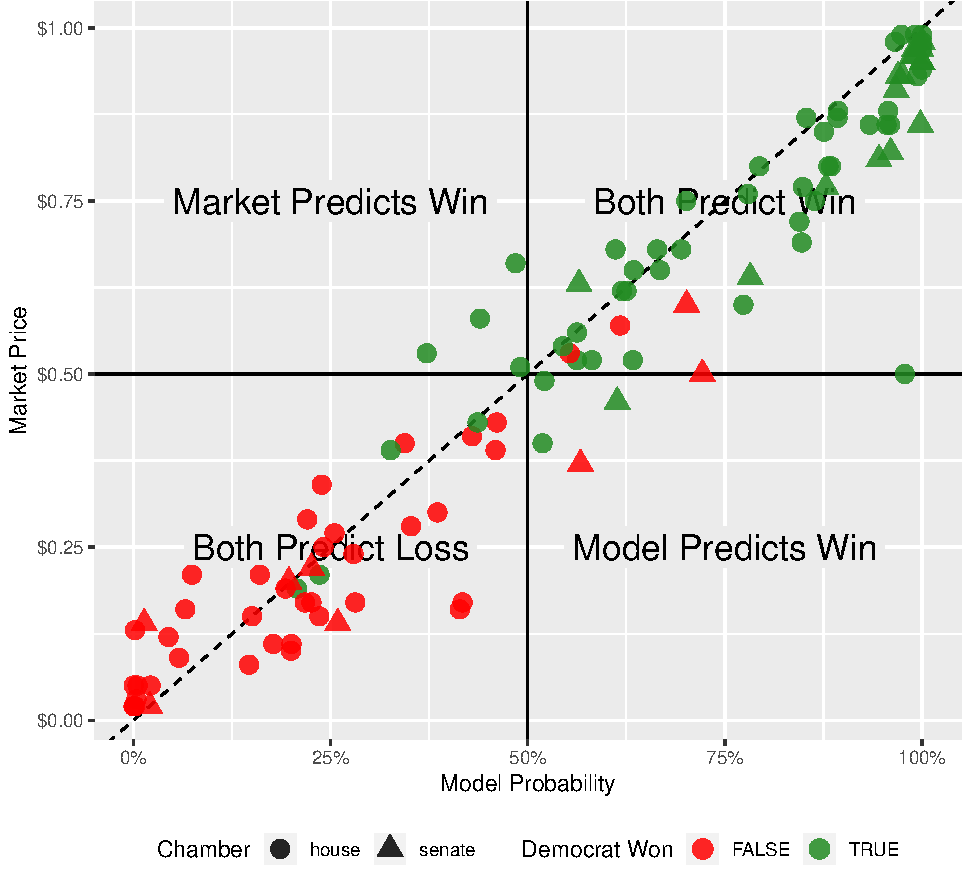
\includegraphics{code_files/figure-latex/plot_cart-1.pdf}

\includegraphics{code_files/figure-latex/plot_nj02-1.pdf}

\includegraphics{code_files/figure-latex/plot_props-1.pdf}

\includegraphics{code_files/figure-latex/plot_calib-1.pdf}

\includegraphics{code_files/figure-latex/plot_brier-1.pdf}

\hypertarget{bibliography}{%
\subsection*{Bibliography}\label{bibliography}}
\addcontentsline{toc}{subsection}{Bibliography}

\hypertarget{refs}{}
\leavevmode\hypertarget{ref-shiny}{}%
Chang, Winston, Joe Cheng, JJ Allaire, Yihui Xie, and Jonathan
McPherson. 2019. \emph{Shiny: Web Application Framework for R}.
\url{https://CRAN.R-project.org/package=shiny}.

\leavevmode\hypertarget{ref-house_district_forecast}{}%
FiveThirtyEight. 2018a. ``House District Forecast.''
\url{https://projects.fivethirtyeight.com/2018-midterm-election-forecast/house/}.

\leavevmode\hypertarget{ref-senate_seat_forecast}{}%
---------. 2018b. ``Senate Seat Forecast.''
\url{https://projects.fivethirtyeight.com/2018-midterm-election-forecast/senate/}.

\leavevmode\hypertarget{ref-forecast_results_2018}{}%
---------. 2018c. ``2018 Midterm Election Results.''
\url{https://53eig.ht/2PiFb0f}.

\leavevmode\hypertarget{ref-lubridate}{}%
Grolemund, Garrett, and Hadley Wickham. 2011. ``Dates and Times Made
Easy with lubridate.'' \emph{Journal of Statistical Software} 40 (3):
1--25. \url{http://www.jstatsoft.org/v40/i03/}.

\leavevmode\hypertarget{ref-legislators_current}{}%
Project, United States. 2018. ``Current Legislators.''
\url{https://theunitedstates.io/congress-legislators/}.

\leavevmode\hypertarget{ref-base}{}%
R Core Team. 2018a. \emph{R: A Language and Environment for Statistical
Computing}. Vienna, Austria: R Foundation for Statistical Computing.
\url{https://www.R-project.org/}.

\leavevmode\hypertarget{ref-stats}{}%
---------. 2018b. \emph{R: A Language and Environment for Statistical
Computing}. Vienna, Austria: R Foundation for Statistical Computing.
\url{https://www.R-project.org/}.

\leavevmode\hypertarget{ref-verification}{}%
Research Applications Laboratory, NCAR -. 2015. \emph{Verification:
Weather Forecast Verification Utilities}.
\url{https://CRAN.R-project.org/package=verification}.

\leavevmode\hypertarget{ref-wayback}{}%
Rudis, Bob. 2017. \emph{Wayback: Tools to Work with Internet Archive
Wayback Machine Apis}. \url{https://github.com/hrbrmstr/wayback}.

\leavevmode\hypertarget{ref-ggplot2}{}%
Wickham, Hadley. 2016. \emph{Ggplot2: Elegant Graphics for Data
Analysis}. Springer-Verlag New York.
\url{https://ggplot2.tidyverse.org}.

\leavevmode\hypertarget{ref-stringr}{}%
---------. 2019. \emph{Stringr: Simple, Consistent Wrappers for Common
String Operations}. \url{https://CRAN.R-project.org/package=stringr}.

\leavevmode\hypertarget{ref-tidyr}{}%
Wickham, Hadley, and Lionel Henry. 2019. \emph{Tidyr: Easily Tidy Data
with 'Spread()' and 'Gather()' Functions}.
\url{https://CRAN.R-project.org/package=tidyr}.

\leavevmode\hypertarget{ref-readr}{}%
Wickham, Hadley, Jim Hester, and Romain Francois. 2018. \emph{Readr:
Read Rectangular Text Data}.
\url{https://CRAN.R-project.org/package=readr}.


\end{document}
